\chapter{Visão Geral} \label{cha:visaogeral}
Neste capítulo, será apresentada uma visão abrangente do projeto do aplicativo \textit{Premium Price}, dividido em quatro seções que abordam diferentes aspectos do projeto.

\section{Contextualização} \label{sec:contextualizacao}

Manter um controle financeiro eficaz atualmente é uma tarefa complicada dada a quantidade de transações que realizamos através dos mais diferentes meios. Porém, ainda sim é uma atividade fundamental para quem deseja prosperar e alcançar seus objetivos pessoais.

Com uma variedade enorme produtos e serviços disponíveis no mercado, encontrar uma opção de qualidade e com preço justo acaba sendo uma tarefa difícil e demorada. Essa abundância de escolhas, embora positiva em termos de variedade, frequentemente resulta em confusão e dificuldade para se tomar boas decisões na hora da compra. Atualmente, os consumidores tendem a ficar sobrecarregados com o grande número de opções à sua disposição e são obrigados a tomar decisões de compra sem confiança \cite{huber2012dazing, nicholls2006purchase}.

Segundo \textcite{heitmann2007effect}, dada a heterogeneidade de gostos entre consumidores, a teoria econômica prevê que uma grande variedade de produtos é benéfica para os clientes e consequentemente resulta em um aumento no número de vendas.

Contudo, de maneira não exclusiva, tal variedade de produtos necessita apresentar certas características para se manter benéfica para grandes escalas. As principais características para que muitas alternativas de produto sejam benéficas é a confiança do consumidor na decisão da compra e a satisfação final, caso contrário, tal variedade pode se tornar algo negativo \cite{schwartz2002maximizing}.

\textcite{tang2017purchase} definem esse impasse como o paradoxo da escolha. Tal paradoxo indica que embora ter muitas escolha possa ser benéfico, também pode causar paralisia e infelicidade nas decisões do cliente, principalmente se a decisão de compra não ter sido feito com certa confiança por parte do cliente. 

Esse fenômeno possui um novo apelido curioso, conhecido como ``efeito Netflix'' ou ``sindrome Netflix'', utilizando a grande plataforma de streaming de video como exemplo, para demonstrar como uma enorme quantidade de opções podem muitas vezes fazer com que o usuário simplesmente não escolha nada. A Netflix inclusive adicionou uma funcionalidade de escolha aleatória para tentar ajudar nesses casos de indecisão \cite{estadao_paradoxo_escolha}.

Os consumidores frequentemente enfrentam o desafio de comparar preços entre diferentes lojas, tanto online quanto físicas, para garantir que estão obtendo o melhor custo-benefício. Esse processo pode ser demorado, tedioso e propenso a erros, especialmente ao lidar com a ampla gama de produtos e preços constantemente alterados. De acordo com \textcite{jung2014online}, os sites de comparação de preços reduzem os custos de pesquisa dos compradores e ajudam na tomada de decisão, fornecendo informações de comparação de preços,
que raramente está presente no contexto de compras físicas no varejo.


Reconhecendo esse problema, a ideia de desenvolver um aplicativo comparador de preços surgiu como uma solução para simplificar a experiência de compra para os consumidores, proporcionando economia de tempo e dinheiro. Ao fornecer, através de uma interface amigável, comparações de preços para produtos em diferentes lojas, o aplicativo permite que os usuários tomem decisões mais acertivas, atendendo às suas necessidades e orçamento. Além disso, o aplicativo deve oferecer recursos como avaliações de usuários e alertas de preço para aprimorar ainda mais a experiência de compra e maximizar as economias para os clientes.


O fácil acesso a uma riqueza de informações de maneira online, torna a Internet um recurso importante mesmo para consumidores que buscam fazer uma compra em uma loja física. Sendo uma comum estrategia entre os consumidores utilizar primariamente a internet como fonte de informação antes de finalizar uma transação ``offline'' \cite{pauwels2011does}. 

Um atleta esta se preparando para uma corrida e quer treinar mais efetivamente utilizando um monitor de frequência cardíaca. Ele decide comprar um Garmin Forerunner 405 HeartRate Monitor. Antes de ir ao shopping mais próximo, ele utiliza algum buscador de preços online, que lista diversas lojas com diferentes preços exatamente do mesmo modelo. Os preços online variam de \$199 a \$299 e também contam com avaliações variando de 1 a 5 estrelas. Mais tarde, o atleta encontra o mesmo monitor num shopping local, custando \$249. Ele se lembra dos vários preços e avaliações que viu online e lembra que tinha alguns em torno de \$ porém com baixa avaliação, e ele decide que o preço no shopping local é razoável e decide finalizar a compra \textcite{bodur2015online}. Neste caso, o consumidor não utilizou exatamente o comparador de preços para buscar o produto, mas mesmo assim o mesmo lhe foi útil para a tomada de uma decisão de compra.

Neste contexto, o presente trabalho tem como objetivo apresentar as informações relativas ao desenvolvimento de um aplicativo comparador de preços que permita aos usuários pesquisar e comparar os preços de diferentes produtos em várias lojas, facilitando e gerando mais confiança na tomada de decisão de compra e proporcionando economia de tempo e dinheiro aos consumidores.

A justificativa para o desenvolvimento desse sistema reside na necessidade de os consumidores lidarem com a crescente variedade de produtos e serviços, seguidos da diversidade e flutuação de preços oferecidos por diferentes lojas. Diversos aplicativos já existem mas específicos para determinados contextos. O aplicativo Premium Price visa ser comparador de preços alimentado pelo próprios usuários, se tornando um aplicativo útil independentemente do contexto do produto ou serviço. 





\section{Descrição do produto do projeto} \label{sec:descricaoproduto}
O aplicativo comparador de preços a ser desenvolvido possui uma série de funcionalidades que visam atender às necessidades dos consumidores em busca de informações precisas e atualizadas sobre os preços de produtos e serviços em diversas lojas. As funcionalidades principais incluem a apresentação organizada e acessível desses dados aos usuário, a capacidade de filtragem nos critérios de busca, avaliações dos produtos e serviços cadastrados e efetivamente o cadastro dos produtos e serviços no aplicativo pelos próprios usuários.

Como se torna algo muito custoso e demorado esperar que os estabelecimentos cadastrem seus produtos, ou que o software faça uma busca pela internet pelos produtos e deixe de encontrar algumas opções, a ideia principal da funcionalidade de buscar produto é que ela possa ser ``alimentada'' pelos próprios usuários. Desse modo, os usuários serão livres para sugerir a edição do valor de algum produto listado no app e/ou adicionar novos produtos. 

Para dar essa liberdade aos usuários é antes preciso garantir a integridade dos dados inseridos, para isso outros usuários poderão avaliar e validar as ações uns dos outros, de modo semelhante como ocorre nos aplicativos de GPS como Google Maps e Waze atualmente. Nestes aplicativos quando alguém sinaliza que há obras em determinado pedaço de um trecho, é enviado uma notificação para todos que estão por perto para validarem a informação. Se a maioria indique que não há obras então a informação enviada inicialmente é ignorada, caso contrário a informação continua a ser mostrada.

Entre as características distintivas do software estão sua interface intuitiva e amigável, a integração com diversas plataformas para login e dispositivos, a possibilidade de receber notificações e alertas de preço, além de funcionalidades avançadas de análise e comparação, como histórico de preços e avaliações de produtos.

Com base nos preços inseridos, o software realizará comparações de preços entre as diferentes lojas, apresentando aos usuários uma visão clara das opções disponíveis e dos melhores preços encontrados. Os usuários também poderão utilizar filtros e categorias para refinar suas buscas, facilitando a localização de produtos específicos e a comparação entre produtos similares.

O software oferecerá a funcionalidade de alertas de preço, permitindo que os usuários recebam notificações quando o preço de um produto de seu interesse atingir um determinado valor pré-definido. Os usuários também terão acesso ao histórico de preços dos produtos, possibilitando acompanhar as variações de preço ao longo do tempo e tomar decisões de compra mais informadas.


\section{Funcionalidades} \label{sec:funcionalidades}

Nesta seção são listados os requisitos funcionais e não funcionais do aplicativo. As funcionalidades são as mesmas tanto no ambiente mobile quanto no ambiente web.

\subsection{REQUISITOS FUNCIONAIS}
\begin{itemize}
  \item Pesquisa de Produtos: Os usuários devem poder pesquisar produtos por nome, categoria ou palavra-chave.
  \item Comparação de Preços: O aplicativo deve comparar os preços dos produtos em diferentes lojas online.
  \item Filtros de Busca: Os usuários devem poder filtrar os resultados da pesquisa por preço, marca, avaliação do produto, entre outros critérios.
  \item Alertas de Preço: Os usuários devem poder configurar alertas para serem notificados quando o preço de um produto atingir um valor desejado.
  \item Histórico de Preços: O aplicativo deve fornecer acesso ao histórico de preços dos produtos, mostrando as variações ao longo do tempo.
  \item Avaliações e Comentários: Os usuários devem poder visualizar e deixar avaliações e comentários sobre os produtos.
  \item Integração com Redes Sociais: O aplicativo deve permitir o compartilhamento de produtos e preços nas redes sociais.
\end{itemize}


\subsection{REQUISITOS NÃO FUNCIONAIS}
\begin{itemize}
  \item Desempenho: O aplicativo deve ter um tempo de resposta rápido e não deve apresentar travamentos durante o uso.
  \item Compatibilidade: O aplicativo deve ser compatível com diferentes dispositivos e sistemas operacionais, como iOS, Android e Web.
  \item Usabilidade: A interface do aplicativo deve ser intuitiva e fácil de usar, mesmo para usuários iniciantes.
  \item Escalabilidade: O aplicativo deve ser capaz de lidar com um grande volume de usuários e produtos sem comprometer o desempenho.
  \item Localização: O aplicativo deve estar disponível em diferentes idiomas e adaptado para diferentes regiões geográficas, considerando variações de preços e moedas.
\end{itemize}


\section{Tecnologias utilizadas} \label{sec:tecnologias}

Para o desenvolvimento de um sistema de comparador de preços, diversas tecnologias são empregadas para os diferentes aspectos do projeto. A figura \autoref{fig:arquitetura} apresenta de um aspecto geral a arquitetura do sistema.

\imagem{Arquitetura do Sistema}{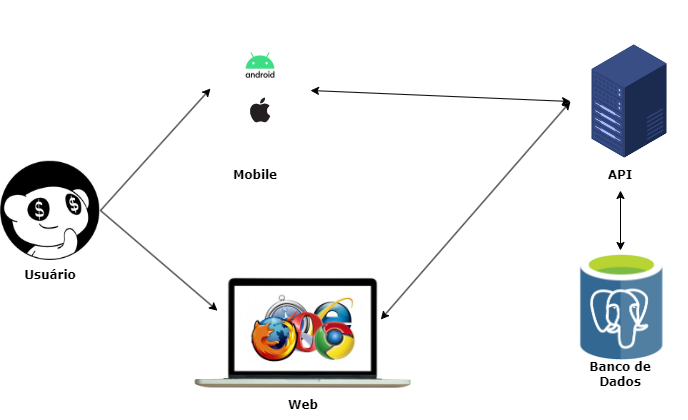
\includegraphics[width = 130mm]{fig/Arquitetura.drawio.png}}{O Autor (2024)}{arquitetura}{nota(s)}{legenda(s)}

Para o desenvolvimento da parte mobile optou-se por utilizar o Flutter, um framework robusto para o desenvolvimento de aplicativos móveis criado pela Google. Para o desenvolvimento web foi escolhido o framework para desenvolvimento de aplicações web Angular. Para a comunicação com o banco de dados optou-se por construir uma API utilizando o Spring, framework de desenvolvimento de aplicações Java. E por fim o banco de dados escolhido foi o PostgreSQL. Abaixo tais tecnologias são apresentadas com mais detalhes.

\subsection{FLUTTER}
Framework de desenvolvimento de aplicativos móveis criado pelo Google. Utiliza a linguagem de programação Dart e permite a criação de interfaces de usuário altamente interativas e responsivas \cite{flutter}.


\subsection{DART}
Dart é uma linguagem orientada a objetos com foco em performance e produtividade, especialmente no desenvolvimento de aplicações web e móveis \cite{dart}.

\subsection{ANGULAR}
Framework de desenvolvimento web mantido pela equipe do Google. É utilizado para construir aplicativos web robustos e escaláveis, utilizando TypeScript como linguagem de programação. Angular também possui recursos para desenvolvimento mobile através do framework Ionic \cite{angular}.

\subsection{SPRING}
Framework de desenvolvimento de aplicações Java, utilizado para criar APIs RESTful e aplicações empresariais escaláveis. É amplamente conhecido pela sua facilidade de configuração e integração, além de oferecer suporte a diversas tecnologias Java como Spring Boot e Spring MVC \cite{spring}.

\subsection{JAVA}
Linguagem de programação amplamente utilizada em desenvolvimento de software, especialmente em aplicações empresariais. Java é conhecido pela sua portabilidade, robustez e segurança, sendo a base para diversos frameworks e tecnologias como Spring, Hibernate e Java EE \cite{java}.

\subsection{POSTGRESQL}
Sistema de gerenciamento de banco de dados relacional de código aberto. É conhecido pela sua confiabilidade, escalabilidade e suporte a recursos avançados como transações ACID e extensões customizadas \cite{postgresql}.

\subsection{HARDWARE}
O hardware utilizado para o desenvolvimento do sistema é um computador somente, com processador AMD Ryzen 5 3600, 16GB de memória RAM, AMD Radeon RX 570 e 1 HD de 1TB de armazenamento.

O sistema operacional utilizado foi o Linux Ubuntu 22. A escolha do Linux como ambiente de desenvolvimento para o aplicativo foi fundamentada em diversos aspectos que favorecem a eficiência, segurança e flexibilidade durante o processo de desenvolvimento. 

Os códigos foram escritos utilizando o editor de texto VSCode, que é amplamente conhecido por sua interface intuitiva e leve, oferecendo uma experiência de desenvolvimento fluida e sem interrupções. Sua ampla gama de extensões e plugins disponíveis no Marketplace permite integrar facilmente com todas as tecnolgias descritas anteriormente.